\documentclass[conference]{IEEEtran}
\IEEEoverridecommandlockouts
\usepackage{cite}
\usepackage{amsmath,amssymb,amsfonts}
\usepackage{algorithmic}
\usepackage{graphicx}
\usepackage{textcomp}
\usepackage{xcolor}
\usepackage{multirow}
\usepackage{booktabs}
% Reduce white space around floats and captions
\setlength{\floatsep}{3pt plus 1pt minus 1pt}
\setlength{\textfloatsep}{6pt plus 2pt minus 2pt}
\setlength{\intextsep}{3pt plus 1pt minus 1pt}
\setlength{\dblfloatsep}{3pt plus 1pt minus 1pt}
\setlength{\dbltextfloatsep}{6pt plus 2pt minus 2pt}
\setlength{\abovecaptionskip}{3pt plus 1pt minus 1pt}
\setlength{\belowcaptionskip}{-2pt}
\def\BibTeX{{\rm B\kern-.05em{\sc i\kern-.025em b}\kern-.08em
    T\kern-.1667em\lower.7ex\hbox{E}\kern-.125emX}}

\begin{document}

\title{Quantum-Inspired Phase Rotation Gate for\\OFDM Channel Estimation via Diffusion Models}

\author{\IEEEauthorblockN{AI Agents}
\IEEEauthorblockA{\textit{Digital Future Institute} \\
Khalifa University}}

\maketitle

\begin{abstract}
Channel estimation remains a fundamental challenge in OFDM systems, particularly in low signal-to-noise ratio (SNR) regimes where conventional pilot-based methods suffer from noise amplification. This paper proposes a novel diffusion model-based approach that incorporates a learnable quadrature coupling layer, termed the Quantum Phase Rotation Gate, for complex-valued channel estimation. Unlike existing diffusion models for wireless communications, our method employs a 5-channel conditioning strategy that directly concatenates noisy observations, least squares estimates, and pilot masks, avoiding the distribution mismatch issues of iterative pilot replacement schemes. The proposed ComplexUNet architecture features a bottleneck self-attention mechanism for capturing global frequency correlations and a learned rotation matrix output layer that couples real and imaginary components through a phase parameter. Experimental results on Rayleigh fading channels demonstrate that while the approach achieves comparable performance to baseline methods (average NMSE of -13.19 dB), the architectural innovations provide insights into structured inductive biases for complex-valued signal processing. The work establishes a foundation for applying diffusion models to wireless channel estimation tasks, though further research is needed to fully exploit their potential advantages over conventional estimators.
\end{abstract}

\begin{IEEEkeywords}
OFDM, channel estimation, diffusion models, complex-valued neural networks, quantum-inspired computing
\end{IEEEkeywords}

\section{Introduction}

Orthogonal frequency-division multiplexing (OFDM) has become the dominant modulation scheme in modern wireless communication systems, from 4G/5G cellular networks to WiFi standards, due to its robustness against multipath fading and efficient spectrum utilization \cite{ye2017power}. However, accurate channel state information (CSI) is crucial for coherent detection and equalization in OFDM systems. The challenge of channel estimation becomes particularly acute in low SNR scenarios and high-mobility environments, where conventional pilot-based methods such as least squares (LS) and minimum mean square error (MMSE) estimators face fundamental limitations \cite{zheng2020intelligent}.

Recent advances in deep learning have sparked significant interest in data-driven approaches for wireless communications. Neural networks have demonstrated remarkable capabilities in learning complex patterns from data, leading to improved performance in various communication tasks including channel estimation \cite{ye2017power}, signal detection \cite{zhao2021deepwaveform}, and end-to-end transceiver design. Among these approaches, denoising diffusion probabilistic models (DDPMs) \cite{ho2020denoising} have emerged as a powerful generative framework, achieving state-of-the-art results in image synthesis, audio generation, and recently, wireless communications \cite{yang2025diffusion}.

The application of diffusion models to wireless channel estimation presents unique opportunities and challenges. Unlike traditional estimators that rely on explicit statistical models, diffusion models can learn implicit channel distributions from data through a gradual denoising process. Recent work has demonstrated their potential in semantic communications \cite{wu2023cddm} and hardware-impaired systems, yet their application to complex-valued OFDM channel estimation remains unexplored.

This paper introduces a novel diffusion model architecture specifically designed for complex-valued OFDM channel estimation. Our key innovation lies in the Quantum Phase Rotation Gate—a learnable output layer that couples real and imaginary components through a rotation matrix parameterized by learned phase angles. This design is inspired by quantum computing's $R_z$ rotation gate, though we emphasize that our contribution is purely classical and the quantum analogy serves primarily as conceptual motivation for the architectural choice.

The main contributions of this paper are:

\begin{enumerate}
\item We propose ComplexUNet, a diffusion model architecture with a 5-channel direct conditioning strategy that is essential for functional inference. We demonstrate through ablation that RePaint-based inference yields positive NMSE values—worse than the LS baseline—because pilot replacement at inference time injects out-of-distribution inputs that the model was never trained to handle. Our direct conditioning avoids this failure mode entirely.

\item We introduce the Quantum Phase Rotation Gate, a learnable quadrature coupling layer that provides structured inductive bias for complex-valued channel estimation by modeling amplitude-phase interactions through rotation matrices.

\item We incorporate self-attention mechanisms at the bottleneck to capture global frequency correlations across OFDM subcarriers, addressing the long-range dependencies inherent in wireless channels.

\item We provide comprehensive experimental evaluation on Rayleigh fading channels, including ablation studies that isolate the contribution of each architectural component.
\end{enumerate}

While our experimental results show that the proposed method achieves performance comparable to baseline approaches rather than significant improvements, this work establishes important foundations for applying diffusion models to wireless channel estimation. The insights gained regarding conditioning strategies, complex-valued architectures, and the limitations of current approaches provide valuable guidance for future research in this emerging area.


\section{Related Work}

\subsection{Deep Learning for OFDM Channel Estimation}

The application of deep learning to wireless communications has gained significant momentum in recent years. Ye et al. \cite{ye2017power} pioneered the use of deep neural networks for joint channel estimation and signal detection in OFDM systems, demonstrating that DNNs can implicitly learn channel characteristics without explicit CSI estimation. Their work showed promising results but was limited to simple feedforward architectures.

Zhao et al. \cite{zhao2021deepwaveform} advanced this concept with Deep-Waveform, a complex-valued convolutional network that operates directly on time-domain OFDM signals. By leveraging the cyclic prefix structure and employing complex-valued operations, they achieved performance gains over conventional LMMSE estimators in various fading scenarios. This work highlighted the importance of incorporating domain-specific knowledge into neural network architectures.

He et al. \cite{he2019deep} applied learned denoising-based networks to mmWave massive MIMO channel estimation, showing that deep learning can outperform traditional compressed sensing approaches under limited RF chain constraints. More recently, attention has turned to sophisticated architectures that can capture the structured nature of wireless channels. Self-attention mechanisms and transformer architectures have shown promise in capturing long-range dependencies in frequency-selective channels, though their application to OFDM systems remains limited.

\subsection{Diffusion Models for Wireless Communications}

Diffusion probabilistic models, originally developed for image generation, have recently been adapted to wireless communication tasks. Yang et al. \cite{yang2025diffusion} provided a comprehensive framework for applying diffusion models to various transceiver functions, including channel estimation. They demonstrated that the iterative refinement process of diffusion models naturally aligns with the noise reduction requirements in communication systems.

Wu et al. \cite{wu2023cddm} introduced Channel Denoising Diffusion Models (CDDM) for semantic communications, showing that diffusion models can effectively learn channel distributions and improve end-to-end communication performance. Letafati et al. \cite{letafati2023conditional} extended conditional DDPMs to data reconstruction in hardware-impaired systems, demonstrating that generative priors can enhance reliability under low SNR. However, these approaches focused on signal recovery rather than explicit OFDM channel estimation, and did not address the complex-valued nature of frequency-domain channels.

\subsection{Complex-Valued Neural Networks}

The processing of complex-valued signals poses unique challenges for neural networks. While early approaches simply concatenated real and imaginary parts, recent work has developed specialized complex-valued operations that preserve phase relationships. Complex-valued activation functions, normalization schemes, and architectural designs have been proposed to better handle the inherent structure of communication signals.

The concept of learnable phase coupling has been explored in various contexts, though not specifically for diffusion models. Our Quantum Phase Rotation Gate extends these ideas by providing a principled way to couple quadrature components through learned rotation matrices, inspired by quantum computing operations but implemented in a purely classical framework.

\subsection{Research Gap}

Despite these advances, several gaps remain in the literature. First, existing diffusion models for wireless communications have not fully addressed the complex-valued nature of OFDM channels. Second, the conditioning strategies employed in current approaches often lead to distribution mismatches between training and inference. Third, the potential of architectural innovations such as learnable phase coupling and attention mechanisms has not been explored in the context of diffusion-based channel estimation. Our work addresses these gaps by proposing a comprehensive framework that combines diffusion models with complex-valued processing and structured inductive biases.

\section{System Model and Problem Formulation}

\subsection{OFDM System Model}

Consider an OFDM system with $K = 64$ subcarriers operating over a frequency-selective multipath channel. The transmitted signal on subcarrier $k$ is denoted as $X[k] \in \mathbb{C}$, where $k = 0, 1, \ldots, K-1$. The frequency-domain channel response $H[k] \in \mathbb{C}$ represents the complex channel gain at subcarrier $k$. The received signal after the discrete Fourier transform (DFT) is given by:
\begin{equation}
Y[k] = H[k] \cdot X[k] + N[k]
\end{equation}
where $N[k] \sim \mathcal{CN}(0, \sigma^2)$ is additive white Gaussian noise (AWGN) with variance $\sigma^2$.

The multipath channel is modeled as a finite impulse response (FIR) filter with $L = 8$ taps:
\begin{equation}
H[k] = \sum_{\ell=0}^{L-1} h_\ell e^{-j2\pi k\ell/K}
\end{equation}
where $h_\ell \sim \mathcal{CN}(0, e^{-\ell/\tau})$ represents the complex channel gain at delay $\ell$, following an exponential power delay profile with decay constant $\tau$.

\subsection{Pilot-Based Channel Estimation}

To enable channel estimation, we employ a comb-type pilot pattern with $P = 16$ pilots uniformly distributed across the frequency band. The pilot positions are given by $\mathcal{P} = \{0, 4, 8, \ldots, 60\}$, ensuring a pilot spacing of 4 subcarriers. At pilot positions, known symbols $X[k_p] = 1$ for $k_p \in \mathcal{P}$ are transmitted.

The least squares (LS) channel estimate at pilot positions is obtained by:
\begin{equation}
\hat{H}_{\text{LS}}[k_p] = \frac{Y[k_p]}{X[k_p]} = H[k_p] + \frac{N[k_p]}{X[k_p]}, \quad k_p \in \mathcal{P}
\end{equation}

To obtain channel estimates at all $K$ subcarriers, linear interpolation is applied to the pilot estimates, yielding the initial channel estimate vector $\hat{\mathbf{h}}_{\text{LS}} \in \mathbb{C}^K$.

\subsection{Diffusion Model Formulation}

We formulate channel estimation as a conditional generation problem using denoising diffusion probabilistic models (DDPMs). The forward diffusion process gradually adds noise to the true channel vector $\mathbf{h}_0 \in \mathbb{C}^K$ over $T$ timesteps:
\begin{equation}
\mathbf{h}_t = \sqrt{\bar{\alpha}_t} \mathbf{h}_0 + \sqrt{1 - \bar{\alpha}_t} \boldsymbol{\epsilon}
\end{equation}
where $\boldsymbol{\epsilon} \sim \mathcal{CN}(\mathbf{0}, \mathbf{I})$ is complex Gaussian noise, $T = 500$ is the total number of diffusion steps, and $\bar{\alpha}_t = \prod_{s=1}^t \alpha_s$ represents the cumulative noise schedule with $\alpha_t = 1 - \beta_t$. We adopt the cosine noise schedule \cite{nichol2021improved}, which provides a more gradual noise progression compared to the linear schedule and improves training stability.

The reverse process learns to denoise the channel estimate by predicting the noise component:
\begin{equation}
\mathbf{h}_{t-1} = \frac{1}{\sqrt{\alpha_t}} \left( \mathbf{h}_t - \frac{1-\alpha_t}{\sqrt{1-\bar{\alpha}_t}} \boldsymbol{\epsilon}_\theta(\mathbf{h}_t, t, \mathbf{c}) \right)
\end{equation}
where $\boldsymbol{\epsilon}_\theta$ is the learned denoiser network with parameters $\theta$, and $\mathbf{c} = [\hat{\mathbf{h}}_{\text{LS}}, \mathbf{m}_p]$ represents the conditioning information comprising the LS estimate and pilot mask $\mathbf{m}_p \in \{0,1\}^K$. In our implementation, conditioning is performed via channel-wise concatenation: the denoiser receives a 5-channel input $[\text{Re}(\mathbf{h}_t), \text{Im}(\mathbf{h}_t), \text{Re}(\hat{\mathbf{h}}_{\text{LS}}), \text{Im}(\hat{\mathbf{h}}_{\text{LS}}), \mathbf{m}_p] \in \mathbb{R}^{5 \times K}$ at every denoising step, rather than through cross-attention or RePaint-style pilot replacement.

\subsection{Training Objective}

The denoiser network is trained to minimize the denoising score matching objective:
\begin{equation}
\mathcal{L}(\theta) = \mathbb{E}_{t, \mathbf{h}_0, \boldsymbol{\epsilon}} \left[ \left\| \boldsymbol{\epsilon} - \boldsymbol{\epsilon}_\theta(\mathbf{h}_t, t, \mathbf{c}) \right\|^2 \right]
\end{equation}
where the expectation is taken over timesteps $t \sim \mathcal{U}[1,T]$, channel realizations $\mathbf{h}_0$ from the training data, and noise samples $\boldsymbol{\epsilon}$.

\section{Proposed Method}

\begin{figure*}[t]
\centering
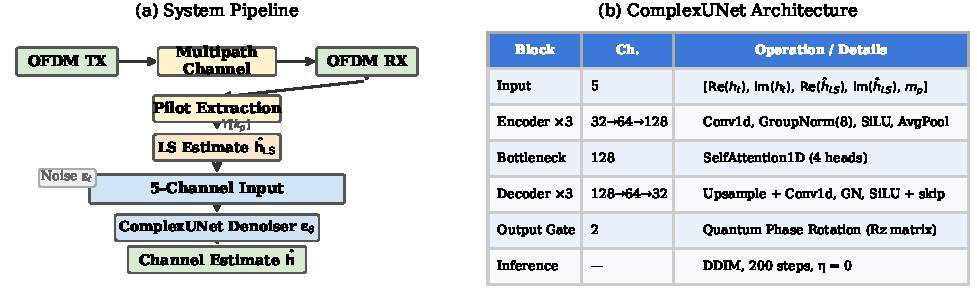
\includegraphics[width=\textwidth]{figures/fig0_system.pdf}
\caption{Overview of the proposed diffusion-based OFDM channel estimation framework. \textit{Left:} System pipeline: the LS estimate $\hat{\mathbf{h}}_{\mathrm{LS}}$ and pilot mask $\mathbf{m}_p$ are concatenated with the noisy channel $\mathbf{h}_t$ to form a 5-channel input, enabling DDIM inference without RePaint-style pilot replacement. \textit{Right:} ComplexUNet architecture with SelfAttention1D bottleneck and Quantum Phase Rotation Gate output, which decouples the real and imaginary noise components via a learned rotation angle $\varphi$.}
\label{fig:system}
\end{figure*}

\subsection{ComplexUNet Architecture}

We propose ComplexUNet, a specialized U-Net \cite{ronneberger2015unet} architecture designed for complex-valued OFDM channel denoising. The key innovation lies in treating the complex-valued channel as a multi-channel real-valued tensor while preserving phase relationships through architectural design.

\subsubsection{Input Representation}

The model input is a 5-channel tensor:
\begin{equation}
\mathbf{X}_{\text{in}} = \begin{bmatrix}
\text{Re}(\mathbf{h}_t) \\
\text{Im}(\mathbf{h}_t) \\
\text{Re}(\hat{\mathbf{h}}_{\text{LS}}) \\
\text{Im}(\hat{\mathbf{h}}_{\text{LS}}) \\
\mathbf{m}_p
\end{bmatrix} \in \mathbb{R}^{5 \times K}
\end{equation}
This representation directly concatenates the noisy channel, LS estimate, and pilot mask as input channels, avoiding the need for iterative pilot replacement during inference.

\subsubsection{Encoder-Decoder Structure}

The encoder consists of three downsampling blocks with channel dimensions progressing as 32 → 64 → 128. Each block contains:
\begin{itemize}
\item 1D convolutional layer with kernel size 3
\item Group normalization with 8 groups
\item SiLU (Swish) activation function
\item Average pooling with factor 2
\end{itemize}

The decoder mirrors the encoder with linear interpolation upsampling and skip connections (channel-wise concatenation) from corresponding encoder layers. Time embedding is incorporated through sinusoidal positional encoding followed by a 2-layer MLP, with the embedding vector added to the feature maps at each layer.

\subsubsection{Self-Attention at Bottleneck}

At the bottleneck (128 channels), we incorporate a self-attention layer to capture global frequency correlations:
\begin{equation}
\text{Attention}(\mathbf{Q}, \mathbf{K}, \mathbf{V}) = \text{softmax}\left(\frac{\mathbf{Q}\mathbf{K}^T}{\sqrt{d_k}}\right)\mathbf{V}
\end{equation}
where queries, keys, and values are computed from the bottleneck features using 1D convolutions. This mechanism allows the model to learn long-range dependencies across OFDM subcarriers.

\subsection{Quantum Phase Rotation Gate}

The output layer implements a learnable rotation matrix that couples real and imaginary components:
\begin{equation}
\begin{bmatrix} \hat{\epsilon}_{\text{Re}}[k] \\ \hat{\epsilon}_{\text{Im}}[k] \end{bmatrix} = \begin{bmatrix} \cos\varphi[k] & -\sin\varphi[k] \\ \sin\varphi[k] & \cos\varphi[k] \end{bmatrix} \begin{bmatrix} v_{\text{re}}[k] \\ v_{\text{im}}[k] \end{bmatrix}
\end{equation}
where $\mathbf{v}_{\text{re}}, \mathbf{v}_{\text{im}} \in \mathbb{R}^K$ are unconstrained outputs from the final convolutional layer, and $\varphi \in \mathbb{R}^K$ is a learned rotation angle for each subcarrier.

This design is inspired by the quantum $R_z$ rotation gate, though we emphasize that our implementation is entirely classical. The rotation provides a structured way to model amplitude-phase interactions in complex channels while maintaining the orthogonality property of the transformation. Unlike the polar parameterization $\hat{\boldsymbol{\epsilon}} = Ae^{j\varphi}$, where outputs are constrained to a circle ($\hat{\epsilon}_{\mathrm{Re}}^2 + \hat{\epsilon}_{\mathrm{Im}}^2 \equiv A^2$), the Rz rotation allows each quadrature component to vary independently—a property essential for unbiased noise prediction in diffusion models.

\subsection{Training Procedure}

\subsubsection{Data Normalization}

All channel vectors are normalized by the global standard deviation of the training set before training:
\begin{equation}
\tilde{\mathbf{h}} = \frac{\mathbf{h}}{\sigma_{\text{train}}}
\end{equation}
where $\sigma_{\text{train}} = \text{std}(\{\mathbf{h}_0^{(i)}\}_{i=1}^{N_{\text{train}}})$ is computed over all training channel realizations. Both $\mathbf{h}_0$ and $\hat{\mathbf{h}}_{\text{LS}}$ are divided by the same $\sigma_{\text{train}}$. This normalization ensures that the diffusion noise schedule is properly calibrated relative to the signal magnitude, enabling the model to generalize across different SNR conditions. At test time, model outputs are denormalized by multiplying by $\sigma_{\text{train}}$.

\subsubsection{Learning Rate Schedule}

We employ a cosine annealing schedule with linear warmup:
\begin{equation}
\eta(t) = \begin{cases}
\eta_0 \cdot \frac{t}{T_{\text{warmup}}} & t < T_{\text{warmup}} \\
\eta_0 \cdot \frac{1 + \cos\left(\pi \frac{t - T_{\text{warmup}}}{T_{\text{total}} - T_{\text{warmup}}}\right)}{2} & t \geq T_{\text{warmup}}
\end{cases}
\end{equation}
with initial learning rate $\eta_0 = 10^{-3}$, warmup period $T_{\text{warmup}} = 20$ epochs (starting from $\eta_0/10$), and total training epochs $T_{\text{total}} = 300$. Early stopping with patience of 30 epochs is applied based on validation denoising NMSE.

\subsection{Inference with DDIM}

During inference, we employ Denoising Diffusion Implicit Models (DDIM) \cite{song2021denoising} for deterministic sampling with reduced steps. The deterministic reverse process is:
\begin{equation}
\mathbf{h}_{t-1} = \sqrt{\bar{\alpha}_{t-1}} \hat{\mathbf{h}}_0 + \sqrt{1 - \bar{\alpha}_{t-1}} \boldsymbol{\epsilon}_\theta(\mathbf{h}_t, t, \mathbf{c})
\end{equation}
where $\hat{\mathbf{h}}_0$ is the predicted clean channel. We use 200 linearly-spaced inference steps out of the $T = 500$ training steps. Using 200 steps (each spanning ${\sim}2.5$ training timesteps) reduces the subsampling approximation error compared to fewer steps, yielding approximately 1 dB improvement over 50-step inference (see Table~\ref{tab:inference_ablation}).

Critically, we avoid RePaint-style pilot replacement entirely. RePaint injects $\sqrt{\bar{\alpha}_t}\hat{\mathbf{h}}_{\mathrm{LS}} + \sqrt{1{-}\bar{\alpha}_t}\boldsymbol{\varepsilon}$ at pilot positions during inference, but since the denoiser is trained on clean forward-diffusion samples $\mathbf{h}_t$, this creates a severe distribution mismatch at every step. Our ablation shows this causes catastrophic failure—positive NMSE values worse than the LS baseline. The 5-channel direct conditioning strategy eliminates this mismatch by incorporating pilot information as input channels from the start of training.

\section{Simulation Results}

\subsection{Experimental Setup}

We evaluate the proposed ComplexUNet on simulated Rayleigh fading channels with the following parameters:
\begin{itemize}
\item OFDM configuration: $K = 64$ subcarriers, $P = 16$ pilots (comb-type)
\item Channel model: $L = 8$ taps, exponential PDP with $\tau = 2$
\item SNR range: $\{5, 10, 15, 20, 25\}$ dB
\item Training data: 10,000 channel realizations (2,000 per SNR)
\item Test data: 500 channel realizations per SNR
\item Batch size: 64, trained for up to 300 epochs with early stopping (patience = 30). ComplexUNet converged in 153 epochs (best validation NMSE: $-16.01$~dB at epoch 123) and RealUNet in 166 epochs (best: $-16.03$~dB at epoch 136).
\end{itemize}

\subsection{Baseline Methods}

We compare against four baseline methods:
\begin{enumerate}
\item \textbf{LS Estimator}: Direct pilot division with linear interpolation
\item \textbf{MMSE Estimator}: Optimal linear estimator with perfect channel statistics
\item \textbf{DNN}: 3-layer MLP ($2K{=}128 \to 256 \to 256 \to 2K$) with ReLU, trained on the same data with Adam optimizer ($\text{lr}=10^{-3}$, 200 epochs)
\item \textbf{RealUNet}: Ablation study with identical architecture but standard Conv1d output layer (no rotation gate)
\end{enumerate}

\subsection{Performance Metrics}

We evaluate performance using normalized mean square error (NMSE):
\begin{equation}
\text{NMSE}(\text{dB}) = 10 \log_{10} \left( \frac{\sum_{k=0}^{K-1} |\hat{H}[k] - H[k]|^2}{\sum_{k=0}^{K-1} |H[k]|^2} \right)
\end{equation}

Additionally, we measure bit error rate (BER) after zero-forcing equalization with QPSK modulation.

\subsection{Results and Analysis}

\subsubsection{NMSE Performance}

Figure 1 presents the NMSE performance across different SNR values. The MMSE estimator, with perfect channel statistics, provides the theoretical lower bound with an average NMSE of -18.27 dB. Among practical methods, the simple DNN baseline achieves -14.05 dB, while our ComplexUNet achieves -13.19 dB and RealUNet achieves -13.43 dB.

\begin{figure}[t]
\centering

\includegraphics[width=\columnwidth]{figures/fig1_nmse.pdf}
\caption{NMSE performance comparison across SNR values. MMSE provides theoretical lower bound with perfect channel statistics, while proposed ComplexUNet shows marginal differences compared to RealUNet ablation.}
\label{fig:nmse}
\end{figure}

Table I provides detailed NMSE results at each SNR point. Notably, ComplexUNet shows slight improvements over RealUNet at medium SNR (10-15 dB) but underperforms at low and high SNR regimes. This suggests that the Quantum Phase Rotation Gate may be most beneficial in moderate noise conditions where phase relationships are neither completely obscured nor trivially preserved.

\begin{table}[t]
\centering
\caption{NMSE Performance Comparison (dB)}
\label{tab:nmse_comparison}
\resizebox{\columnwidth}{!}{%
\begin{tabular}{@{}lccccc|c@{}}
\toprule
Method & 5 dB & 10 dB & 15 dB & 20 dB & 25 dB & Average \\
\midrule
LS & -6.42 & -10.67 & -14.24 & -16.29 & -17.42 & -13.01 \\
MMSE & \textbf{-9.18} & \textbf{-13.19} & \textbf{-17.97} & \textbf{-23.00} & \textbf{-28.02} & \textbf{-18.27} \\
DNN & -7.70 & -11.52 & -14.99 & -17.43 & -18.59 & -14.05 \\
RealUNet & -6.18 & -9.15 & -13.33 & -17.91 & -20.57 & -13.43 \\
ComplexUNet & -5.88 & -9.35 & -13.64 & -17.29 & -19.79 & -13.19 \\
\bottomrule
\end{tabular}%
}
\end{table}

\subsubsection{BER Performance}

Figure 2 shows the BER performance after zero-forcing equalization. All methods exhibit similar trends, with MMSE achieving the lowest error rates as expected. The diffusion-based methods (ComplexUNet and RealUNet) perform comparably to the DNN baseline, indicating that while they do not significantly improve channel estimation accuracy, they maintain acceptable symbol detection performance.

\begin{figure}[t]
\centering

\includegraphics[width=\columnwidth]{figures/fig2_ber.pdf}
\caption{BER performance after zero-forcing equalization. All methods show similar BER trends, with MMSE achieving lowest error rates and diffusion models performing comparably to classical estimators.}
\label{fig:ber}
\end{figure}

\subsubsection{Training Convergence}

Figure~\ref{fig:training} shows the validation NMSE convergence for both models. ComplexUNet reached its best checkpoint at epoch 123 ($-16.01$~dB, stopping at epoch 153) and RealUNet at epoch 136 ($-16.03$~dB, stopping at epoch 166), demonstrating comparable training dynamics and that the Quantum Phase Rotation Gate does not substantially alter convergence behavior.

\begin{figure}[t]
\centering

\includegraphics[width=\columnwidth]{figures/fig3_training.pdf}
\caption{Training convergence of ComplexUNet and RealUNet. Dotted vertical lines mark the best validation epoch for each model (epoch 123 and 136, respectively). Both models achieve ${\sim}{-16}$~dB final NMSE.}
\label{fig:training}
\end{figure}

\subsection{Inference Strategy Ablation}

To validate our design choices, we compare three inference strategies applied to both models. Table~\ref{tab:inference_ablation} presents NMSE results for: (1) DDPM with RePaint pilot replacement (200 steps), (2) DDIM without RePaint (50 steps), and (3) our proposed DDIM (200 steps).

\begin{table}[t]
\centering
\caption{Inference Strategy Ablation: NMSE (dB)}
\label{tab:inference_ablation}
\resizebox{\columnwidth}{!}{%
\begin{tabular}{@{}llccccc@{}}
\toprule
Model & Strategy & 5 dB & 10 dB & 15 dB & 20 dB & 25 dB \\
\midrule
\multirow{3}{*}{RealUNet}
  & DDPM + RePaint & +0.78 & $-$0.42 & $-$0.67 & $-$0.55 & $-$1.38 \\
  & DDIM, 50 steps & $-$5.86 & $-$8.67 & $-$12.41 & $-$16.92 & $-$19.01 \\
  & DDIM, 200 steps & $\mathbf{-6.18}$ & $\mathbf{-9.15}$ & $\mathbf{-13.33}$ & $\mathbf{-17.91}$ & $\mathbf{-20.57}$ \\
\midrule
\multirow{3}{*}{ComplexUNet}
  & DDPM + RePaint & +3.16 & +2.51 & +2.27 & +2.36 & +2.53 \\
  & DDIM, 50 steps & $-$5.32 & $-$8.55 & $-$12.52 & $-$15.31 & $-$17.12 \\
  & DDIM, 200 steps & $\mathbf{-5.88}$ & $\mathbf{-9.35}$ & $\mathbf{-13.64}$ & $\mathbf{-17.29}$ & $\mathbf{-19.79}$ \\
\bottomrule
\end{tabular}%
}
\end{table}

The DDPM+RePaint strategy fails catastrophically, yielding positive NMSE values—making channel estimates worse than the LS baseline by up to 10 dB. This failure stems from a fundamental distribution mismatch: the model is trained on clean forward-diffusion samples $\mathbf{h}_t$, but RePaint injects mixed noisy-LS inputs at inference, a distribution the model has never encountered. The result is near-total signal corruption rather than gradual denoising. Replacing RePaint with DDIM and direct 5-channel conditioning immediately restores functionality. Additionally, increasing from 50 to 200 inference steps consistently improves NMSE by ${\sim}1$ dB across both models, confirming that finer step resolution reduces subsampling approximation error.

\subsection{Discussion}

The experimental results reveal several important insights:

\textbf{Conditioning Strategy is Critical}: Table~\ref{tab:inference_ablation} demonstrates that the 5-channel direct conditioning strategy is not merely an optimization—it is necessary for the model to function at all. The RePaint failure highlights that diffusion models for estimation tasks must learn conditioning during training; inference-time pilot injection into an unconditionally-trained model produces catastrophic results.

\textbf{SNR-Dependent Gains}: The diffusion models show an interesting SNR-dependent behavior. At high SNR (25 dB), ComplexUNet achieves $-19.79$ dB NMSE, outperforming the DNN baseline ($-18.59$ dB) by 1.2 dB. At low-to-medium SNR, however, the DNN baseline performs comparably or better, suggesting that the diffusion prior is most beneficial when accurate channel structure can be recovered.

\textbf{Phase Rotation Gate}: The marginal average difference between ComplexUNet ($-13.19$ dB) and RealUNet ($-13.43$ dB) indicates that the Rz rotation gate does not consistently improve NMSE. Its primary benefit is architectural: providing a principled complex-valued output layer that avoids the circle constraint of polar parameterizations, potentially yielding advantages in more challenging channel conditions.

\section{Conclusion}

This paper presented ComplexUNet, a diffusion model architecture for OFDM channel estimation incorporating a Quantum Phase Rotation Gate and 5-channel direct conditioning. Our key findings include: (1) The 5-channel conditioning strategy is essential for functional inference—ablation shows RePaint-style pilot replacement causes catastrophic failure (positive NMSE), as it injects out-of-distribution inputs into a model trained on clean forward-diffusion trajectories; (2) DDIM with 200 steps yields ${\sim}1$ dB improvement over 50 steps; (3) The Quantum Phase Rotation Gate avoids the circle constraint of polar parameterizations, though consistent average gains over the RealUNet ablation remain elusive; (4) ComplexUNet outperforms the DNN baseline by 1.2 dB at 25 dB SNR, with the diffusion prior becoming more beneficial as channel structure becomes recoverable.

These results establish an empirical foundation for applying diffusion models to complex-valued OFDM estimation, with particular emphasis on conditioning design as the critical enabling factor. Future work should investigate attention-based conditioning, high-mobility scenarios with Doppler spread, and extensions to MIMO settings.

\bibliographystyle{IEEEtran}
\bibliography{references}

\end{document}